\part{Inhomogenous ODEs; Fourier Transforms}
\section{Dirac delta function}

\begin{definition}[Dirac Delta Function]
	We define a generalised function $\delta(x - \xi)$ such that
	\begin{align}
		\begin{aligned} \label{eq:6.1}
			&\delta(x-\xi) = 0 \ \ \forall \; x \neq \xi; \\
			&\int_{-\infty}^\infty \delta(x-\xi) \dd{x} = 1.
		\end{aligned} 	
	\end{align} 
	% \begin{enumerate}
	% 	\item $\delta(x-\xi) = 0$ for all $x \neq \xi$;
	% 	\item $\int_{-\infty}^\infty \delta(x-\xi) \dd{x} = 1$.
	% \end{enumerate}
	This acts as a linear operator $\int \dd{x} \delta(x - \xi)$ on some arbitrary function $f(x)$ to produce a number $f(\xi)$.
	\begin{align} \label{eq:6.2}
		\int_{-\infty}^\infty \dd{x} \delta(x-\xi) f(x) = f(\xi)
	\end{align}
	This relationship holds provided that $f(x)$ is sufficiently `well-behaved' at $x=\xi$ and $x\to\pm \infty$.
\end{definition}

\begin{note}
	\begin{itemize}
		\item Strictly, the $\delta$ `function' is classified as a distribution, not as a function.
		See lectures notes of Jozsa and Skinner section 6.1 for more details.
		\item For this reason, we will never use $\delta$ outside an integral, although such an integral may be implied.
		\item The $\delta$ function represents a unit point source (e.g. mass, charge) or an impulse.
	\end{itemize} 
\end{note}

\subsection{Some limiting approximations}

A discrete approximation as $n \to \infty$ is $\delta_n = \begin{cases}
	0 & x > \frac{1}{n} \\
	\frac{n}{2} & |x| \leq \frac{1}{n} \\
	0 & x < - \frac{1}{n}
\end{cases}$.
\begin{figure}[h] 
    \centering 
    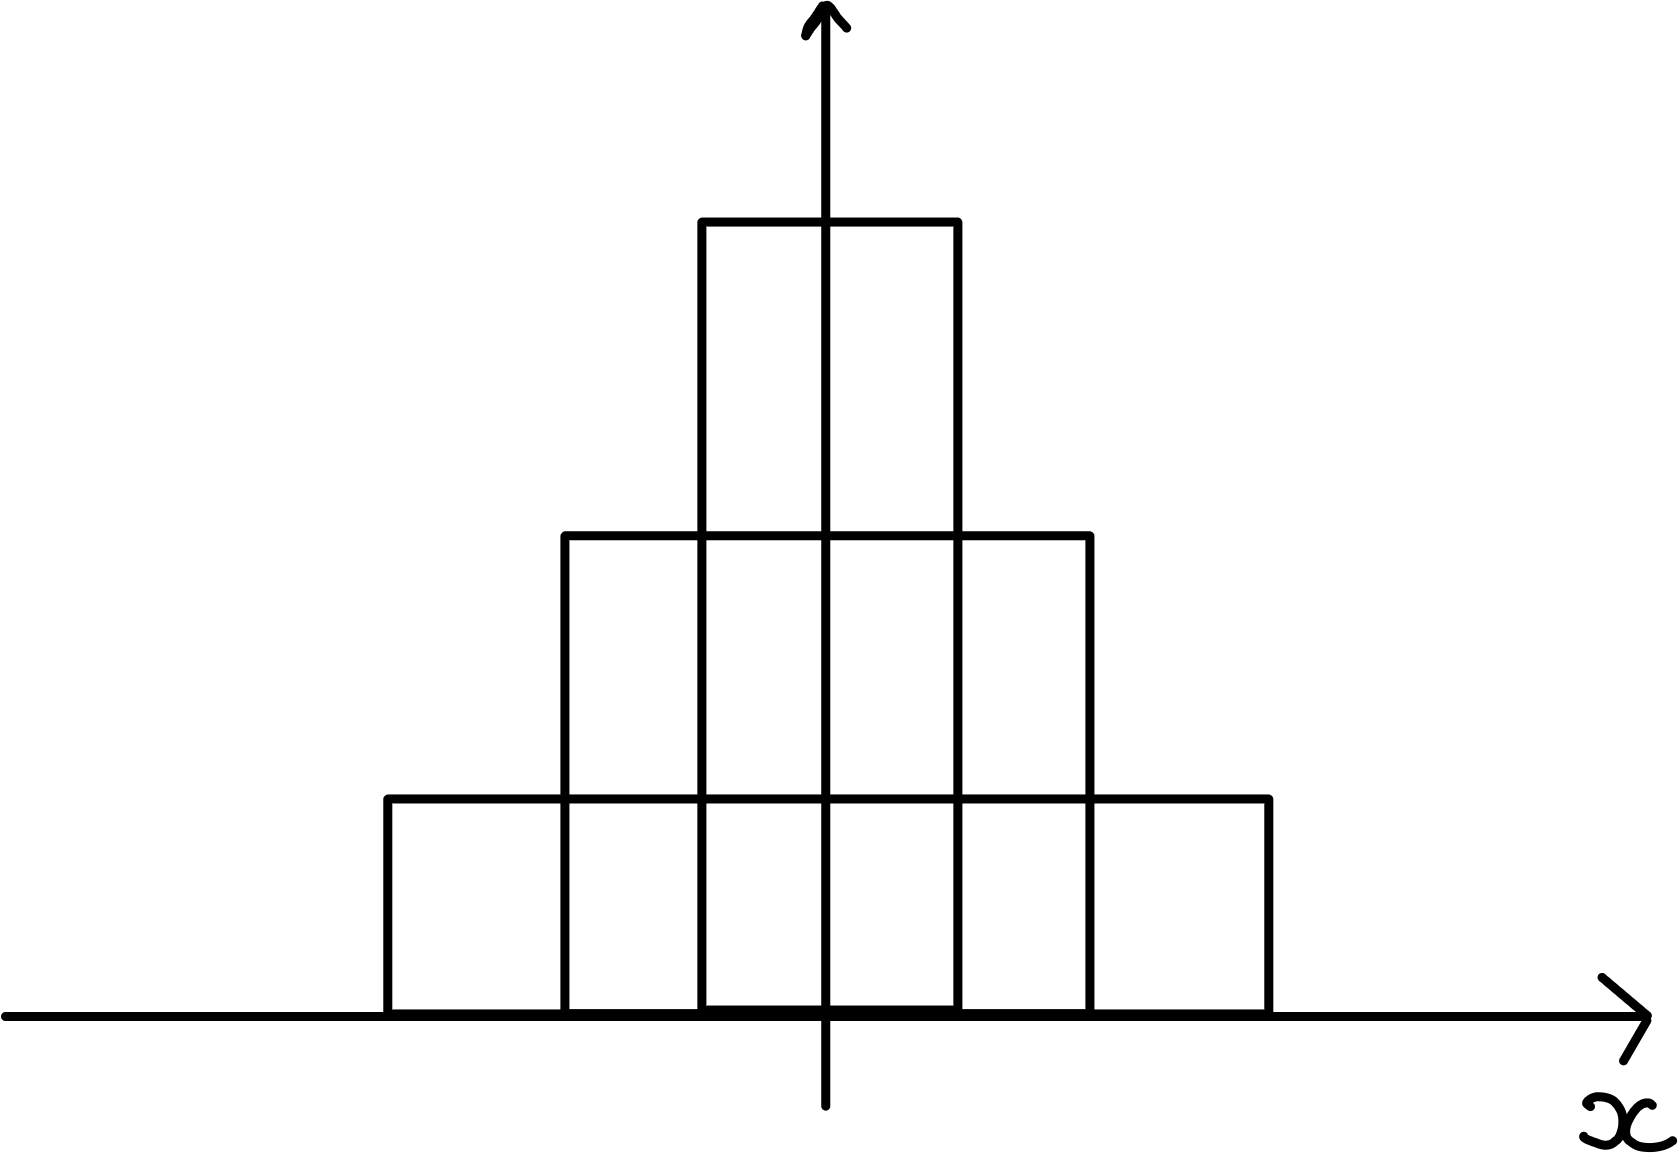
\includegraphics[height=5cm]{06-discretedelta} 
	\caption{Discrete approximation}
\end{figure}

\underline{Continuous:}
We can approximate the $\delta$ function using a Gaussian approximation as $\epsilon \to 0$.
\begin{align} \label{eq:6.3}
	\delta_\varepsilon(x) = \frac{1}{\varepsilon \sqrt{\pi}} \exp[-\frac{x^2}{\varepsilon^2}]
\end{align}
Therefore verifying \cref{eq:6.2},
\begin{align*}
	\int_{-\infty}^\infty f(x) \delta(x) \dd{x} & = \lim_{\varepsilon \to 0} \int_{-\infty}^\infty \frac{1}{\varepsilon \sqrt{\pi}} \exp[-\frac{x^2}{\varepsilon^2}] f(x) \dd{x}
	\intertext{Let $y = \frac{x}{\epsilon}$,}
    & = \lim_{\varepsilon \to 0} \int_{-\infty}^\infty \frac{1}{\sqrt{\pi}} \exp[-y^2] f(\varepsilon y) \dd{y} \\
    & = \lim_{\varepsilon \to 0} \int_{-\infty}^\infty \frac{1}{\sqrt{\pi}} \exp[-y^2] [f(0) + \varepsilon y f'(0) + \cdots] \dd{y} \\
    & = f(0)
\end{align*}
for all `well-behaved functions' $f$ at $0, \pm \infty$\footnote{Well behaved at $0$ lets us taylor expand and well behaved at $\pm \infty$ means it doesn't diverge faster than the Gaussian.}.
\begingroup
\tikzset{every picture/.style={scale=0.8}}
\begin{center}
	% Recommended preamble:
% \usetikzlibrary{arrows.meta}
% \usetikzlibrary{backgrounds}
% \usepgfplotslibrary{patchplots}
% \usepgfplotslibrary{fillbetween}
% \pgfplotsset{%
%     layers/standard/.define layer set={%
%         background,axis background,axis grid,axis ticks,axis lines,axis tick labels,pre main,main,axis descriptions,axis foreground%
%     }{
%         grid style={/pgfplots/on layer=axis grid},%
%         tick style={/pgfplots/on layer=axis ticks},%
%         axis line style={/pgfplots/on layer=axis lines},%
%         label style={/pgfplots/on layer=axis descriptions},%
%         legend style={/pgfplots/on layer=axis descriptions},%
%         title style={/pgfplots/on layer=axis descriptions},%
%         colorbar style={/pgfplots/on layer=axis descriptions},%
%         ticklabel style={/pgfplots/on layer=axis tick labels},%
%         axis background@ style={/pgfplots/on layer=axis background},%
%         3d box foreground style={/pgfplots/on layer=axis foreground},%
%     },
% }

\begin{tikzpicture}[/tikz/background rectangle/.style={fill={rgb,1:red,1.0;green,1.0;blue,1.0}, draw opacity={1.0}}, show background rectangle]
\begin{axis}[point meta max={nan}, point meta min={nan}, legend cell align={left}, legend columns={1}, title={}, title style={at={{(0.5,1)}}, anchor={south}, font={{\fontsize{14 pt}{18.2 pt}\selectfont}}, color={rgb,1:red,0.0;green,0.0;blue,0.0}, draw opacity={1.0}, rotate={0.0}, align={center}}, legend style={color={rgb,1:red,0.0;green,0.0;blue,0.0}, draw opacity={1.0}, line width={1}, solid, fill={rgb,1:red,1.0;green,1.0;blue,1.0}, fill opacity={1.0}, text opacity={1.0}, font={{\fontsize{8 pt}{10.4 pt}\selectfont}}, text={rgb,1:red,0.0;green,0.0;blue,0.0}, cells={anchor={center}}, at={(1.02, 1)}, anchor={north west}}, axis background/.style={fill={rgb,1:red,1.0;green,1.0;blue,1.0}, opacity={1.0}}, anchor={north west}, xshift={1.0mm}, yshift={-1.0mm}, width={145.4mm}, height={99.6mm}, scaled x ticks={false}, xlabel={$x$}, x tick style={color={rgb,1:red,0.0;green,0.0;blue,0.0}, opacity={1.0}}, x tick label style={color={rgb,1:red,0.0;green,0.0;blue,0.0}, opacity={1.0}, rotate={0}}, xlabel style={at={(ticklabel cs:0.5)}, anchor=near ticklabel, at={{(ticklabel cs:0.5)}}, anchor={near ticklabel}, font={{\fontsize{11 pt}{14.3 pt}\selectfont}}, color={rgb,1:red,0.0;green,0.0;blue,0.0}, draw opacity={1.0}, rotate={0.0}}, xmajorgrids={true}, xmin={-3.18}, xmax={3.18}, xticklabels={{$-3$,$-2$,$-1$,$0$,$1$,$2$,$3$}}, xtick={{-3.0,-2.0,-1.0,0.0,1.0,2.0,3.0}}, xtick align={inside}, xticklabel style={font={{\fontsize{8 pt}{10.4 pt}\selectfont}}, color={rgb,1:red,0.0;green,0.0;blue,0.0}, draw opacity={1.0}, rotate={0.0}}, x grid style={color={rgb,1:red,0.0;green,0.0;blue,0.0}, draw opacity={0.1}, line width={0.5}, solid}, axis x line*={left}, x axis line style={color={rgb,1:red,0.0;green,0.0;blue,0.0}, draw opacity={1.0}, line width={1}, solid}, scaled y ticks={false}, ylabel={$\delta_\varepsilon(x)$}, y tick style={color={rgb,1:red,0.0;green,0.0;blue,0.0}, opacity={1.0}}, y tick label style={color={rgb,1:red,0.0;green,0.0;blue,0.0}, opacity={1.0}, rotate={0}}, ylabel style={at={(ticklabel cs:0.5)}, anchor=near ticklabel, at={{(ticklabel cs:0.5)}}, anchor={near ticklabel}, font={{\fontsize{11 pt}{14.3 pt}\selectfont}}, color={rgb,1:red,0.0;green,0.0;blue,0.0}, draw opacity={1.0}, rotate={0.0}}, ymajorgrids={true}, ymin={-0.1354047167432424}, ymax={4.6488952748513235}, yticklabels={{$0$,$1$,$2$,$3$,$4$}}, ytick={{0.0,1.0,2.0,3.0,4.0}}, ytick align={inside}, yticklabel style={font={{\fontsize{8 pt}{10.4 pt}\selectfont}}, color={rgb,1:red,0.0;green,0.0;blue,0.0}, draw opacity={1.0}, rotate={0.0}}, y grid style={color={rgb,1:red,0.0;green,0.0;blue,0.0}, draw opacity={0.1}, line width={0.5}, solid}, axis y line*={left}, y axis line style={color={rgb,1:red,0.0;green,0.0;blue,0.0}, draw opacity={1.0}, line width={1}, solid}, colorbar={false}]
    \addplot[color={rgb,1:red,0.0;green,0.6056;blue,0.9787}, name path={9301c92f-18de-4450-ae5a-35afff11106c}, draw opacity={1.0}, line width={1}, solid]
        table[row sep={\\}]
        {
            \\
            -3.0  3.1687901131724237e-250  \\
            -2.9609367239208475  9.39781460355311e-244  \\
            -2.5997403313265086  6.293312116930993e-188  \\
            -2.3826763547775043  7.2292706182272e-158  \\
            -2.199151525136937  1.7029524963311301e-134  \\
            -1.9997921198677944  3.149477195036373e-111  \\
            -1.8160003818614874  9.796570654868876e-92  \\
            -1.6189562143740408  6.363369594192493e-73  \\
            -1.3906612226458708  7.961352563788823e-54  \\
            -1.1877795755559142  2.7604528396966285e-39  \\
            -1.00987065383912  2.0335438369458794e-28  \\
            -0.8159021733787222  1.4177079603549339e-18  \\
            -0.6207808849887516  8.774963089119262e-11  \\
            -0.5129151172455673  2.1988390791159464e-7  \\
            -0.40504934950238297  0.00012426653351608005  \\
            -0.3793914604421633  0.0004505922462812648  \\
            -0.3537335713819437  0.0015018170599526582  \\
            -0.3280756823217241  0.004601020214025313  \\
            -0.30241779326150453  0.012956718933280433  \\
            -0.28958884873139473  0.021066476676521728  \\
            -0.27675990420128493  0.033538197898531213  \\
            -0.26393095967117514  0.05228035000074701  \\
            -0.25110201514106534  0.07979729999477607  \\
            -0.24468754287601044  0.09780975191093307  \\
            -0.23827307061095554  0.11925836598538044  \\
            -0.23185859834590064  0.14464661959675607  \\
            -0.22544412608084574  0.1745180932892  \\
            -0.21902965381579084  0.20945241252217625  \\
            -0.21261518155073594  0.2500593001870305  \\
            -0.20620070928568104  0.29697055637461756  \\
            -0.19978623702062615  0.35082982805772434  \\
            -0.19311667417481276  0.4148896941616267  \\
            -0.18644711132899938  0.48786086723146954  \\
            -0.179777548483186  0.5704091975261611  \\
            -0.17310798563737262  0.6631385200082948  \\
            -0.16643842279155924  0.7665653624099615  \\
            -0.15976885994574586  0.8810921405607898  \\
            -0.15643407852283917  0.9426057726481537  \\
            -0.15309929709993247  1.0069795778232735  \\
            -0.14976451567702576  1.0742194972115524  \\
            -0.14642973425411906  1.144319235495385  \\
            -0.13976017140830568  1.2930071712466085  \\
            -0.1330906085624923  1.452719842937036  \\
            -0.12642104571667892  1.6228934357221645  \\
            -0.11975148287086554  1.8027078023619365  \\
            -0.11308192002505216  1.9910761630477771  \\
            -0.10641235717923878  2.1866416071706682  \\
            -0.0997427943334254  2.387781273641675  \\
            -0.093073231487612  2.5926188605085754  \\
            -0.0864036686417986  2.7990458343279454  \\
            -0.07973410579598522  3.004751384501715  \\
            -0.07306454295017184  3.2072608106018317  \\
            -0.06639498010435846  3.403981657691705  \\
            -0.05972541725854508  3.5922565442186114  \\
            -0.053055854412731696  3.769421278914807  \\
            -0.049721072989825005  3.8530180581228444  \\
            -0.046386291566918314  3.932866557163835  \\
            -0.04305151014401162  4.008659584009742  \\
            -0.03971672872110493  4.080101282195823  \\
            -0.03638194729819824  4.146909048087371  \\
            -0.03304716587529155  4.20881538861213  \\
            -0.02971238445238486  4.265569702415517  \\
            -0.026377603029478166  4.316939967872759  \\
            -0.02304282160657147  4.3627143220667  \\
            -0.01970804018366478  4.402702515706628  \\
            -0.01637325876075809  4.43673723001371  \\
            -0.0130384773378514  4.464675242821175  \\
            -0.009703695914944709  4.486398432518669  \\
            -0.006368914492038016  4.501814609993881  \\
            -0.003034133069131324  4.510858170372357  \\
            0.0003006483537753681  4.5134905581080815  \\
            0.00363542977668206  4.5097005408109965  \\
            0.006970211199588752  4.499504289090081  \\
            0.010304992622495443  4.482945261617806  \\
            0.013639774045402136  4.460093896559111  \\
            0.016446949680120546  4.436050532649423  \\
            0.019254125314838957  4.407688634459925  \\
            0.02206130094955737  4.37509281648702  \\
            0.02486847658427578  4.33835987017029  \\
            0.027675652218994193  4.297598285088465  \\
            0.030482827853712605  4.252927715223899  \\
            0.033290003488431016  4.204478393969637  \\
            0.03609717912314943  4.152390501880297  \\
            0.03890435475786784  4.096813491460039  \\
            0.04171153039258625  4.037905373535479  \\
            0.044518706027304664  3.975831969976599  \\
            0.047325881662023075  3.910766137703177  \\
            0.0529402329314599  3.772378973628859  \\
            0.05855458420089672  3.624236630985895  \\
            0.06416893547033355  3.467891779126281  \\
            0.06978328673977037  3.3049301678273997  \\
            0.0753976380092072  3.1369442410579933  \\
            0.08101198927864402  2.9655078064457685  \\
            0.09224069181751766  2.6183451713407653  \\
            0.10346939435639131  2.274813343838524  \\
            0.10908374562582812  2.1075449324561104  \\
            0.11469809689526494  1.9447137211070167  \\
            0.12031244816470177  1.7872375274579795  \\
            0.1259267994341386  1.635899546742392  \\
            0.13154115070357542  1.4913471540850294  \\
            0.13715550197301224  1.354093421221986  \\
            0.14276985324244906  1.224521083222509  \\
            0.1483842045118859  1.1028886478129494  \\
            0.1539985557813227  0.9893383101111929  \\
            0.15961290705075953  0.8839053188399951  \\
            0.16522725832019636  0.7865284357532991  \\
            0.17084160958963318  0.6970611370233241  \\
            0.17645596085907  0.6152832223133685  \\
            0.18207031212850683  0.540912522581052  \\
            0.18768466339794365  0.4736164295543675  \\
            0.19329901466738048  0.41302300647863943  \\
            0.20015350120732034  0.3475472888688286  \\
            0.20700798774726023  0.2906977972981577  \\
            0.21386247428720012  0.24168948238753776  \\
            0.22071696082713999  0.19973857025202604  \\
            0.22757144736707985  0.1640794897023623  \\
            0.2344259339070197  0.1339784136076442  \\
            0.24128042044695958  0.10874355839981903  \\
            0.24813490698689947  0.08773248361983058  \\
            0.2618438800667792  0.05608396573600284  \\
            0.27555285314665895  0.03500013384385919  \\
            0.28926182622653873  0.021323249741359636  \\
            0.30297079930641846  0.012682059321306555  \\
            0.33038874546617797  0.004173694427288526  \\
            0.3578066916259375  0.001247562501897781  \\
            0.38522463778569693  0.00033869966713932266  \\
            0.41264258394545644  8.351760293801774e-5  \\
            0.513108876864534  2.1710397507607256e-7  \\
            0.6135751697836116  1.5504732924613018e-10  \\
            0.7991519189555105  8.007717307674473e-18  \\
            0.9871354150600441  3.717119866523065e-27  \\
            1.1978122140406555  5.9668426120590896e-40  \\
            1.388719406219134  1.1245970773344658e-53  \\
            1.6072949743767582  7.069478227687967e-72  \\
            1.8096765128752679  4.2497444897081354e-91  \\
            2.009200994923107  2.8171737950880423e-112  \\
            2.202922753671847  5.885372290691178e-135  \\
            2.4015123274889874  2.2613412180743035e-160  \\
            2.6190902607646405  9.818482143595239e-191  \\
            2.93515789239279  1.576481105264437e-239  \\
            3.0  3.1687901131724237e-250  \\
        }
        ;
    \addlegendentry {$ε = 2^{-3}$}
    \addplot[color={rgb,1:red,0.8889;green,0.4356;blue,0.2781}, name path={c21cbeaa-296f-451f-bd6a-41d8ce7bbebc}, draw opacity={1.0}, line width={1}, solid]
        table[row sep={\\}]
        {
            \\
            -3.0  6.532503647797609e-63  \\
            -2.9609367239208475  2.7108969603874276e-61  \\
            -2.5997403313265086  2.4523141841736653e-47  \\
            -2.3826763547775043  8.028416833972961e-40  \\
            -2.199151525136937  5.59315591241414e-34  \\
            -1.9997921198677944  3.667886677676559e-28  \\
            -1.8160003818614874  2.739206736675871e-23  \\
            -1.6189562143740408  1.3828595696209478e-18  \\
            -1.3906612226458708  8.22437693647071e-14  \\
            -1.1877795755559142  3.548962213099155e-10  \\
            -1.00987065383912  1.8489266275542406e-7  \\
            -0.9128864136089211  3.6533856380411288e-6  \\
            -0.8159021733787222  5.3426040225238017e-5  \\
            -0.7671218512812296  0.00018379573787953506  \\
            -0.718341529183737  0.0005859339883465548  \\
            -0.6695612070862442  0.0017309827946840215  \\
            -0.6207808849887516  0.004738791675832074  \\
            -0.5938144430529555  0.00800314998834751  \\
            -0.5668480011171595  0.013205299090033602  \\
            -0.5398815591813634  0.02128773595372286  \\
            -0.5129151172455673  0.033527768877876  \\
            -0.49943189627766926  0.041711179769700395  \\
            -0.4859486753097712  0.05159098028925014  \\
            -0.47246545434187315  0.06344078863434087  \\
            -0.45898223337397515  0.07755983076081178  \\
            -0.4454990124060771  0.09427110964857881  \\
            -0.43201579143817903  0.11391839882946726  \\
            -0.41853257047028103  0.13686191481366292  \\
            -0.40504934950238297  0.16347255038032008  \\
            -0.3922204049722732  0.1925383125101431  \\
            -0.3793914604421633  0.22558084589558128  \\
            -0.3665625159120535  0.26290570927544793  \\
            -0.3537335713819437  0.30479690355339456  \\
            -0.3409046268518339  0.351506872659441  \\
            -0.3280756823217241  0.4032457767357382  \\
            -0.31524673779161433  0.46017028518452024  \\
            -0.30241779326150453  0.5223721945981948  \\
            -0.28958884873139473  0.5898672291426873  \\
            -0.27675990420128493  0.6625844251972072  \\
            -0.26393095967117514  0.740356534547053  \\
            -0.25110201514106534  0.8229118979356298  \\
            -0.23827307061095554  0.9098682404590356  \\
            -0.22544412608084574  1.0007288199057438  \\
            -0.21261518155073594  1.0948813173160676  \\
            -0.19978623702062615  1.1915997953932551  \\
            -0.17310798563737262  1.3971960727303163  \\
            -0.14642973425411906  1.601375175864644  \\
            -0.1330906085624923  1.6998153997686394  \\
            -0.11975148287086554  1.7940627411561616  \\
            -0.11308192002505216  1.8391970454076139  \\
            -0.10641235717923878  1.8827848463136836  \\
            -0.0997427943334254  1.9246640207897956  \\
            -0.093073231487612  1.9646760967652295  \\
            -0.0864036686417986  2.002667245688309  \\
            -0.07973410579598522  2.038489263013643  \\
            -0.07306454295017184  2.0720005279739997  \\
            -0.06639498010435846  2.1030669339731616  \\
            -0.05972541725854508  2.1315627810699223  \\
            -0.053055854412731696  2.1573716222573904  \\
            -0.046386291566918314  2.180387055574678  \\
            -0.03971672872110493  2.2005134545171066  \\
            -0.03304716587529155  2.2176666297321503  \\
            -0.026377603029478166  2.2317744155958645  \\
            -0.01970804018366478  2.2427771759517907  \\
            -0.0130384773378514  2.2506282240531252  \\
            -0.006368914492038016  2.255294152570284  \\
            0.0003006483537753681  2.256755070399699  \\
            0.006970211199588752  2.255004743924887  \\
            0.013639774045402136  2.250050641325983  \\
            0.019254125314838957  2.2434119001468  \\
            0.02486847658427578  2.23453769803537  \\
            0.030482827853712605  2.2234547356111407  \\
            0.03609717912314943  2.210196259399388  \\
            0.04171153039258625  2.1948018956702997  \\
            0.047325881662023075  2.1773174531274493  \\
            0.0529402329314599  2.157794695820574  \\
            0.05855458420089672  2.136291087858008  \\
            0.06416893547033355  2.1128695116804703  \\
            0.06978328673977037  2.0875979618286604  \\
            0.0753976380092072  2.060549216290819  \\
            0.08101198927864402  2.0318004876518745  \\
            0.08662634054808084  2.0014330563819547  \\
            0.09224069181751766  1.9695318886981033  \\
            0.09785504308695449  1.936185241508368  \\
            0.10346939435639131  1.901484257001622  \\
            0.11469809689526494  1.8283957870374044  \\
            0.1259267994341386  1.7510375135454417  \\
            0.13715550197301224  1.6701998846137278  \\
            0.1483842045118859  1.5866794937157722  \\
            0.17084160958963318  1.4147314556915325  \\
            0.19329901466738048  1.2412231106901714  \\
            0.20700798774726023  1.1368855002785407  \\
            0.22071696082713999  1.0350748981349687  \\
            0.2344259339070197  0.9367312311771446  \\
            0.24813490698689947  0.8426483957719927  \\
            0.2618438800667792  0.7534700102840881  \\
            0.27555285314665895  0.6696898529332199  \\
            0.2824073396865988  0.6299385084806262  \\
            0.28926182622653873  0.591656500823318  \\
            0.2961163127664786  0.5548660682714782  \\
            0.30297079930641846  0.5195815694201555  \\
            0.3098252858463583  0.48580988934316116  \\
            0.3166797723862982  0.4535508745804794  \\
            0.3235342589262381  0.422797791297742  \\
            0.33038874546617797  0.3935378011219317  \\
            0.33724323200611783  0.365752449338727  \\
            0.34409771854605775  0.3394181603677886  \\
            0.3509522050859976  0.3145067357064409  \\
            0.3578066916259375  0.2909858498431189  \\
            0.3715156647058172  0.2479686857928801  \\
            0.38522463778569693  0.2100438571036372  \\
            0.39893361086557666  0.17685254090600896  \\
            0.41264258394545644  0.14801331912672744  \\
            0.42520087056034117  0.12507983481737658  \\
            0.43775915717522584  0.10516761620100935  \\
            0.4503174437901105  0.08798020924749983  \\
            0.4628757304049952  0.0732312050342449  \\
            0.47543401701987986  0.06064787662928307  \\
            0.4879923036347646  0.04997390067616607  \\
            0.5005505902496493  0.04097124186992212  \\
            0.513108876864534  0.03342129210016576  \\
            0.5382254500943033  0.02190464106419405  \\
            0.5633420233240728  0.014069606920156238  \\
            0.5884585965538423  0.00885647101039307  \\
            0.6135751697836116  0.005463517830428291  \\
            0.6599693570765863  0.0021227912726021004  \\
            0.7063635443695611  0.0007698907850036368  \\
            0.7527577316625358  0.000260638068680944  \\
            0.7991519189555105  8.236325006182906e-5  \\
            0.8931436670077773  6.463365888678688e-6  \\
            0.9871354150600441  3.823032005475622e-7  \\
            1.1978122140406555  2.419872242587979e-10  \\
            1.388719406219134  8.966140292320151e-14  \\
            1.6072949743767582  2.5246613567124797e-18  \\
            1.8096765128752679  3.953183710873427e-23  \\
            2.009200994923107  2.0059019581202498e-28  \\
            2.202922753671847  4.288444336583017e-34  \\
            2.4015123274889874  1.898662693160747e-40  \\
            2.6190902607646405  4.8737963792137843e-48  \\
            2.93515789239279  3.0851656321409415e-60  \\
            3.0  6.532503647797609e-63  \\
        }
        ;
    \addlegendentry {$ε = 2^{-2}$}
    \addplot[color={rgb,1:red,0.2422;green,0.6433;blue,0.3044}, name path={a532c86f-34d5-401a-a2f8-fbea3ee3ae0c}, draw opacity={1.0}, line width={1}, solid]
        table[row sep={\\}]
        {
            \\
            -3.0  2.617301239249265e-16  \\
            -2.9609367239208475  6.642966284232493e-16  \\
            -2.5997403313265086  2.0486974321776623e-12  \\
            -2.3826763547775043  1.5496773083759404e-10  \\
            -2.199151525136937  4.4771127021678465e-9  \\
            -1.9997921198677944  1.274053815791314e-7  \\
            -1.8160003818614874  2.1061533944186058e-6  \\
            -1.6189562143740408  3.1570271401773835e-5  \\
            -1.3906612226458708  0.0004930143351068951  \\
            -1.2892203991008926  0.0014625486533025077  \\
            -1.1877795755559142  0.003995849654926455  \\
            -1.1433023451267155  0.006049505342491231  \\
            -1.098825114697517  0.009014829881361682  \\
            -1.0543478842683185  0.013222761125996624  \\
            -1.00987065383912  0.019090342266493098  \\
            -0.9856245937815703  0.02316665956020944  \\
            -0.9613785337240206  0.027981477577716036  \\
            -0.9371324736664708  0.03363840512206885  \\
            -0.9128864136089211  0.04024923912705927  \\
            -0.8886403535513714  0.047933316468420556  \\
            -0.8643942934938216  0.05681654327252581  \\
            -0.8401482334362719  0.06703006834805664  \\
            -0.8159021733787222  0.07870857365915374  \\
            -0.7915120123299759  0.09207214494911897  \\
            -0.7671218512812296  0.1071933033317097  \\
            -0.7427316902324832  0.12420532735226801  \\
            -0.718341529183737  0.14323394985453056  \\
            -0.6939513681349906  0.16439359323483554  \\
            -0.6695612070862442  0.18778330714435104  \\
            -0.645171046037498  0.21348248717841992  \\
            -0.6207808849887516  0.2415464726583744  \\
            -0.6072976640208536  0.2580867337408062  \\
            -0.5938144430529555  0.2753588470813796  \\
            -0.5803312220850575  0.2933599071654701  \\
            -0.5668480011171595  0.3120835346184055  \\
            -0.5398815591813634  0.3516544878165147  \\
            -0.5129151172455673  0.3939444252252405  \\
            -0.4859486753097712  0.43876021496303963  \\
            -0.45898223337397515  0.4858397098643159  \\
            -0.43201579143817903  0.5348503244708183  \\
            -0.40504934950238297  0.5853896035231857  \\
            -0.3537335713819437  0.6840477728467939  \\
            -0.30241779326150453  0.7826702181130658  \\
            -0.27675990420128493  0.8306041589298587  \\
            -0.25110201514106534  0.8768435889087651  \\
            -0.23827307061095554  0.8991422846901173  \\
            -0.22544412608084574  0.9207948833793353  \\
            -0.21261518155073594  0.9417281595091707  \\
            -0.19978623702062615  0.9618700463688094  \\
            -0.18644711132899938  0.9818979823452749  \\
            -0.17310798563737262  1.000917159203043  \\
            -0.15976885994574586  1.0188534059570384  \\
            -0.14642973425411906  1.0356358328408293  \\
            -0.1330906085624923  1.0511972968814627  \\
            -0.11975148287086554  1.0654748486148982  \\
            -0.10641235717923878  1.0784101557909305  \\
            -0.093073231487612  1.0899499000818593  \\
            -0.07973410579598522  1.1000461430226183  \\
            -0.06639498010435846  1.108656657669609  \\
            -0.053055854412731696  1.1157452227683253  \\
            -0.03971672872110493  1.121281876562594  \\
            -0.026377603029478166  1.1252431277569246  \\
            -0.0130384773378514  1.1276121215534636  \\
            0.0003006483537753681  1.1283787591213756  \\
            0.013639774045402136  1.127539769313673  \\
            0.02486847658427578  1.1255912724766708  \\
            0.03609717912314943  1.1225133259931799  \\
            0.047325881662023075  1.1183152160096705  \\
            0.05855458420089672  1.1130095807653564  \\
            0.06978328673977037  1.1066123472024472  \\
            0.08101198927864402  1.099142651309606  \\
            0.09224069181751766  1.0906227427561608  \\
            0.10346939435639131  1.0810778744821823  \\
            0.11469809689526494  1.07053617801115  \\
            0.1259267994341386  1.0590285253466782  \\
            0.13715550197301224  1.046588378401896  \\
            0.1483842045118859  1.033251626988803  \\
            0.15961290705075953  1.0190564164646698  \\
            0.17084160958963318  1.0040429661927324  \\
            0.18207031212850683  0.988253380024656  \\
            0.19329901466738048  0.9717314500521467  \\
            0.20700798774726023  0.9506331997835771  \\
            0.22071696082713999  0.928595852737249  \\
            0.2344259339070197  0.9057066272881538  \\
            0.24813490698689947  0.8820544496124538  \\
            0.27555285314665895  0.8328220693321566  \\
            0.30297079930641846  0.7816228191133114  \\
            0.3578066916259375  0.6761635619529811  \\
            0.41264258394545644  0.5710300917052741  \\
            0.43775915717522584  0.5242691501916592  \\
            0.4628757304049952  0.47891433947534506  \\
            0.4879923036347646  0.43528089703145695  \\
            0.513108876864534  0.3936312819616734  \\
            0.5382254500943033  0.35417494150272855  \\
            0.5633420233240728  0.3170693677492819  \\
            0.5884585965538423  0.28242229115391515  \\
            0.6135751697836116  0.2502948344319125  \\
            0.636772263430099  0.22287740227971747  \\
            0.6599693570765863  0.19761077387712192  \\
            0.6831664507230737  0.17445588803290002  \\
            0.7063635443695611  0.1533525761175881  \\
            0.7295606380160484  0.1342230030339914  \\
            0.7527577316625358  0.11697505492611515  \\
            0.7759548253090232  0.1015055983314776  \\
            0.7991519189555105  0.08770354832240959  \\
            0.8226498559685772  0.07530348193074325  \\
            0.8461477929816439  0.06437164018665043  \\
            0.8696457299947106  0.05478424944888236  \\
            0.8931436670077773  0.04641928867032293  \\
            0.9166416040208439  0.039158213485873776  \\
            0.9401395410339106  0.03288735015795745  \\
            0.9636374780469774  0.02749897579691534  \\
            0.9871354150600441  0.022892107624872673  \\
            1.039804614805197  0.014935829170435485  \\
            1.0924738145503499  0.009530921186095772  \\
            1.1451430142955026  0.005948430622595685  \\
            1.1978122140406555  0.0036310472895996586  \\
            1.2932658101298946  0.0014026898210219914  \\
            1.388719406219134  0.0005037733370112364  \\
            1.6072949743767582  3.6697339416610036e-5  \\
            1.8096765128752679  2.3084503853856095e-6  \\
            2.009200994923107  1.095623203067123e-7  \\
            2.202922753671847  4.189466672366105e-9  \\
            2.4015123274889874  1.0806766051757937e-10  \\
            2.6190902607646405  1.3678883186240157e-12  \\
            2.93515789239279  1.2201224461958778e-15  \\
            3.0  2.617301239249265e-16  \\
        }
        ;
    \addlegendentry {$ε = 2^{-1}$}
    \addplot[color={rgb,1:red,0.7644;green,0.4441;blue,0.8243}, name path={3d3b8db3-3875-4af1-b985-df233926b873}, draw opacity={1.0}, line width={1}, solid]
        table[row sep={\\}]
        {
            \\
            -3.0  6.962652597337395e-5  \\
            -2.9804683619604235  7.825353142176361e-5  \\
            -2.9609367239208475  8.788238021458185e-5  \\
            -2.780338527623678  0.0002478598057309385  \\
            -2.5997403313265086  0.00065490869221132  \\
            -2.4912083430520067  0.0011379988527388208  \\
            -2.3826763547775043  0.0019313972881056679  \\
            -2.2909139399572207  0.0029656720142803637  \\
            -2.199151525136937  0.004477759929072768  \\
            -2.0994718225023656  0.006873052994034807  \\
            -1.9997921198677944  0.010342088314832028  \\
            -1.9078962508646409  0.014810290333855728  \\
            -1.8160003818614874  0.020853732502639676  \\
            -1.7667393399896256  0.024878959359024413  \\
            -1.717478298117764  0.029537440601296816  \\
            -1.6682172562459026  0.03489841881497424  \\
            -1.6189562143740408  0.04103277394919611  \\
            -1.5618824664419981  0.04920097778986362  \\
            -1.5048087185099557  0.05861209395382674  \\
            -1.4477349705779132  0.06936995099885265  \\
            -1.3906612226458708  0.08156919674941943  \\
            -1.3399408108733817  0.09368601820811569  \\
            -1.2892203991008926  0.10705054419689662  \\
            -1.2384999873284035  0.12169380775138758  \\
            -1.1877795755559142  0.13763015014866012  \\
            -1.1433023451267155  0.15266562674138  \\
            -1.098825114697517  0.16867498597533834  \\
            -1.0543478842683185  0.1856272953488789  \\
            -1.00987065383912  0.2034767196475148  \\
            -0.9613785337240206  0.223887042688019  \\
            -0.9128864136089211  0.2451888504807545  \\
            -0.8643942934938216  0.2672575610177068  \\
            -0.8159021733787222  0.2899457914674334  \\
            -0.718341529183737  0.3367617757529399  \\
            -0.6207808849887516  0.383761562557319  \\
            -0.5668480011171595  0.40914666245985226  \\
            -0.5129151172455673  0.43368064341086626  \\
            -0.4859486753097712  0.44552092745808314  \\
            -0.45898223337397515  0.457019310764875  \\
            -0.43201579143817903  0.4681331162970862  \\
            -0.40504934950238297  0.4788202952497445  \\
            -0.3793914604421633  0.4885551959575023  \\
            -0.3537335713819437  0.49783211242185793  \\
            -0.3280756823217241  0.5066177035268725  \\
            -0.30241779326150453  0.5148799745506462  \\
            -0.27675990420128493  0.5225884707336694  \\
            -0.25110201514106534  0.5297144639203194  \\
            -0.22544412608084574  0.5362311306762859  \\
            -0.19978623702062615  0.5421137203388033  \\
            -0.17310798563737262  0.5475336721076567  \\
            -0.14642973425411906  0.5522211880375654  \\
            -0.11975148287086554  0.5561566050821904  \\
            -0.093073231487612  0.5593233276647973  \\
            -0.06639498010435846  0.5617079442556648  \\
            -0.03971672872110493  0.5633003219916456  \\
            -0.0130384773378514  0.5640936784037662  \\
            0.013639774045402136  0.5640846295423769  \\
            0.03609717912314943  0.563454919682847  \\
            0.05855458420089672  0.5622584933491559  \\
            0.08101198927864402  0.5604989637139971  \\
            0.10346939435639131  0.558181635179785  \\
            0.1259267994341386  0.5553134767359842  \\
            0.1483842045118859  0.55190308704106  \\
            0.17084160958963318  0.5479606514739062  \\
            0.19329901466738048  0.543497891454965  \\
            0.22071696082713999  0.5373632769935863  \\
            0.24813490698689947  0.5304997060701915  \\
            0.27555285314665895  0.5229369807883504  \\
            0.30297079930641846  0.514707630054979  \\
            0.33038874546617797  0.5058466767154356  \\
            0.3578066916259375  0.4963913895970638  \\
            0.38522463778569693  0.4863810229140504  \\
            0.41264258394545644  0.4758565455777577  \\
            0.4628757304049952  0.45538189394277423  \\
            0.513108876864534  0.43359443539317166  \\
            0.5633420233240728  0.41077109004719264  \\
            0.6135751697836116  0.38719012330447605  \\
            0.7063635443695611  0.34255796328191324  \\
            0.7991519189555105  0.297896629807229  \\
            0.8461477929816439  0.27573058522420135  \\
            0.8931436670077773  0.2540890322173566  \\
            0.9401395410339106  0.23311408745127576  \\
            0.9871354150600441  0.21292798466826043  \\
            1.039804614805197  0.19136769824711208  \\
            1.0924738145503499  0.17103894867209235  \\
            1.1451430142955026  0.15202391026764628  \\
            1.1978122140406555  0.1343752468565796  \\
            1.245539012085275  0.1195844606537621  \\
            1.2932658101298946  0.10593798549484941  \\
            1.3409926081745143  0.09342221462253296  \\
            1.388719406219134  0.08201061965345743  \\
            1.44336329825854  0.07025227733704982  \\
            1.4980071902979462  0.05982148000526454  \\
            1.552651082337352  0.05063610971817858  \\
            1.6072949743767582  0.04260591960138823  \\
            1.6578903590013856  0.036117947179541934  \\
            1.708485743626013  0.030461597742526946  \\
            1.7590811282506404  0.025559879632634452  \\
            1.8096765128752679  0.021337396869379504  \\
            1.8595576333872277  0.017768651343759368  \\
            1.9094387538991873  0.014723339873807988  \\
            1.959319874411147  0.012139395202251348  \\
            2.009200994923107  0.009959249307842357  \\
            2.106061874297477  0.006685183887720753  \\
            2.202922753671847  0.004404037251619891  \\
            2.3022175405804175  0.002815626323588246  \\
            2.4015123274889874  0.0017649614997523278  \\
            2.5103012941268137  0.0010343546945692393  \\
            2.6190902607646405  0.0005920030701929997  \\
            2.7771240765787155  0.0002523274069904906  \\
            2.93515789239279  0.00010230860264657333  \\
            2.967578946196395  8.448895477786285e-5  \\
            3.0  6.962652597337395e-5  \\
        }
        ;
    \addlegendentry {$ε = 2^{0}$}
\end{axis}
\end{tikzpicture}

\end{center} 
\endgroup

\underline{Further Examples}
We could alternatively use the Dirichlet kernel (as $n \to \infty$)
\begin{align} \label{eq:6.4}
	\delta_n(x) = \frac{\sin n x}{\pi x} = \frac{1}{2\pi} \int_{-n}^n e^{ikx} \dd{k}
\end{align}
or even
\begin{align} \label{eq:6.5}
	\delta_n(x) = \frac{n}{2} \sech^2 nx
\end{align}

\subsection{Integral and derivative of delta function}
\subsubsection{Integral of $\delta(x)$}
We define the Heaviside step function by
\begin{align} \label{eq:6.6}
	H(x) = \begin{cases}
		1 & x \geq 0 \\
		0 & x < 0
	\end{cases}
\end{align}
For $x \neq 0$, we have
\begin{align} \label{eq:6.7}
	H(x) = \int_{-\infty}^x \delta(t) \dd{t}
\end{align}
Thus,
\begin{align*}
	\dv{x} H(x) = \delta(x)
\end{align*}
where this identification takes place under an implied integral.

\begin{exercise}
	Verify using \cref{eq:6.5} $\delta(x) = \lim_{n \to \infty} \frac{n}{2} \sech^2 nx$ [You will find $\frac{1}{2} (\tanh nx + 1)$ which is an approximate step function. This also gives $H(0) = \frac{1}{2}$ (an alternative definition)].
\end{exercise} 

\subsubsection{Derivative of $\delta(x)$}
We define $\delta'(x)$ using integration by parts.
\begin{align}
	\int_{-\infty}^\infty \delta'(x-\xi) f(x) \dd{x} &= \qty[\delta(x-\xi) f(x)]_{-\infty}^\infty - \int_{-\infty}^\infty \delta(x-\xi) f'(x) \dd{x} \notag \\
    &= - \int_{-\infty}^\infty \delta(x-\xi) f'(x) \dd{x} \notag \\
    \int_{-\infty}^\infty \delta'(x-\xi) f(x) \dd{x} &= - f'(\xi) \label{eq:6.8}
\end{align}
This is valid for all $f$ that are smooth at $x = \xi$.
\begin{example}
	Consider the Gaussian approximation \cref{eq:6.3}:
	\begin{align*}
		\delta_\varepsilon(x) = \frac{1}{\varepsilon \sqrt{\pi}} \exp[-\frac{x^2}{\varepsilon^2}]
	\end{align*}
	Then,
	\begin{align*}
		\delta_\varepsilon'(x) = \frac{-2x}{\varepsilon^3 \sqrt{\pi}} \exp[-\frac{x^2}{\varepsilon^2}]
	\end{align*}

	\begingroup
	\tikzset{every picture/.style={scale=0.8}}
	\begin{center}
		% Recommended preamble:
% \usetikzlibrary{arrows.meta}
% \usetikzlibrary{backgrounds}
% \usepgfplotslibrary{patchplots}
% \usepgfplotslibrary{fillbetween}
% \pgfplotsset{%
%     layers/standard/.define layer set={%
%         background,axis background,axis grid,axis ticks,axis lines,axis tick labels,pre main,main,axis descriptions,axis foreground%
%     }{
%         grid style={/pgfplots/on layer=axis grid},%
%         tick style={/pgfplots/on layer=axis ticks},%
%         axis line style={/pgfplots/on layer=axis lines},%
%         label style={/pgfplots/on layer=axis descriptions},%
%         legend style={/pgfplots/on layer=axis descriptions},%
%         title style={/pgfplots/on layer=axis descriptions},%
%         colorbar style={/pgfplots/on layer=axis descriptions},%
%         ticklabel style={/pgfplots/on layer=axis tick labels},%
%         axis background@ style={/pgfplots/on layer=axis background},%
%         3d box foreground style={/pgfplots/on layer=axis foreground},%
%     },
% }

\begin{tikzpicture}[/tikz/background rectangle/.style={fill={rgb,1:red,1.0;green,1.0;blue,1.0}, draw opacity={1.0}}, show background rectangle]
\begin{axis}[point meta max={nan}, point meta min={nan}, legend cell align={left}, legend columns={1}, title={}, title style={at={{(0.5,1)}}, anchor={south}, font={{\fontsize{14 pt}{18.2 pt}\selectfont}}, color={rgb,1:red,0.0;green,0.0;blue,0.0}, draw opacity={1.0}, rotate={0.0}, align={center}}, legend style={color={rgb,1:red,0.0;green,0.0;blue,0.0}, draw opacity={1.0}, line width={1}, solid, fill={rgb,1:red,1.0;green,1.0;blue,1.0}, fill opacity={1.0}, text opacity={1.0}, font={{\fontsize{8 pt}{10.4 pt}\selectfont}}, text={rgb,1:red,0.0;green,0.0;blue,0.0}, cells={anchor={center}}, at={(1.02, 1)}, anchor={north west}}, axis background/.style={fill={rgb,1:red,1.0;green,1.0;blue,1.0}, opacity={1.0}}, anchor={north west}, xshift={1.0mm}, yshift={-1.0mm}, width={145.4mm}, height={99.6mm}, scaled x ticks={false}, xlabel={$x$}, x tick style={color={rgb,1:red,0.0;green,0.0;blue,0.0}, opacity={1.0}}, x tick label style={color={rgb,1:red,0.0;green,0.0;blue,0.0}, opacity={1.0}, rotate={0}}, xlabel style={at={(ticklabel cs:0.5)}, anchor=near ticklabel, at={{(ticklabel cs:0.5)}}, anchor={near ticklabel}, font={{\fontsize{11 pt}{14.3 pt}\selectfont}}, color={rgb,1:red,0.0;green,0.0;blue,0.0}, draw opacity={1.0}, rotate={0.0}}, xmajorgrids={true}, xmin={-3.18}, xmax={3.18}, xticklabels={{$-3$,$-2$,$-1$,$0$,$1$,$2$,$3$}}, xtick={{-3.0,-2.0,-1.0,0.0,1.0,2.0,3.0}}, xtick align={inside}, xticklabel style={font={{\fontsize{8 pt}{10.4 pt}\selectfont}}, color={rgb,1:red,0.0;green,0.0;blue,0.0}, draw opacity={1.0}, rotate={0.0}}, x grid style={color={rgb,1:red,0.0;green,0.0;blue,0.0}, draw opacity={0.1}, line width={0.5}, solid}, axis x line*={left}, x axis line style={color={rgb,1:red,0.0;green,0.0;blue,0.0}, draw opacity={1.0}, line width={1}, solid}, scaled y ticks={false}, ylabel={$\delta'_\varepsilon(x)$}, y tick style={color={rgb,1:red,0.0;green,0.0;blue,0.0}, opacity={1.0}}, y tick label style={color={rgb,1:red,0.0;green,0.0;blue,0.0}, opacity={1.0}, rotate={0}}, ylabel style={at={(ticklabel cs:0.5)}, anchor=near ticklabel, at={{(ticklabel cs:0.5)}}, anchor={near ticklabel}, font={{\fontsize{11 pt}{14.3 pt}\selectfont}}, color={rgb,1:red,0.0;green,0.0;blue,0.0}, draw opacity={1.0}, rotate={0.0}}, ymajorgrids={true}, ymin={-32.82592937325758}, ymax={32.82305373414853}, yticklabels={{$-30$,$-20$,$-10$,$0$,$10$,$20$,$30$}}, ytick={{-30.0,-20.0,-10.0,0.0,10.0,20.0,30.0}}, ytick align={inside}, yticklabel style={font={{\fontsize{8 pt}{10.4 pt}\selectfont}}, color={rgb,1:red,0.0;green,0.0;blue,0.0}, draw opacity={1.0}, rotate={0.0}}, y grid style={color={rgb,1:red,0.0;green,0.0;blue,0.0}, draw opacity={0.1}, line width={0.5}, solid}, axis y line*={left}, y axis line style={color={rgb,1:red,0.0;green,0.0;blue,0.0}, draw opacity={1.0}, line width={1}, solid}, colorbar={false}]
    \addplot[color={rgb,1:red,0.0;green,0.6056;blue,0.9787}, name path={f792d4e5-906c-4b99-a42b-d00e0e8d42ec}, draw opacity={1.0}, line width={1}, solid]
        table[row sep={\\}]
        {
            \\
            -3.0  1.2168154034582108e-247  \\
            -2.9609367239208475  3.5617708011852854e-241  \\
            -2.5997403313265086  2.0942050979854476e-185  \\
            -2.3826763547775043  2.2048015570352257e-155  \\
            -2.199151525136937  4.79366474181422e-132  \\
            -1.9997921198677944  8.061823585711441e-109  \\
            -1.8160003818614874  2.27719373442239e-89  \\
            -1.6189562143740408  1.3186581438562247e-70  \\
            -1.3906612226458708  1.4171576691549956e-51  \\
            -1.1877795755559142  4.196876162914533e-37  \\
            -1.00987065383912  2.6286287926106213e-26  \\
            -0.8159021733787222  1.4805900877694795e-16  \\
            -0.6207808849887516  6.972581570825069e-9  \\
            -0.5129151172455673  1.4436067892081802e-5  \\
            -0.40504934950238297  0.00644276205639735  \\
            -0.3793914604421633  0.02188170884871219  \\
            -0.3537335713819437  0.06799911835896122  \\
            -0.3409046268518339  0.11591856042158305  \\
            -0.3280756823217241  0.19321380429982715  \\
            -0.31524673779161433  0.3148543419621841  \\
            -0.30241779326150453  0.5015478205071646  \\
            -0.28958884873139473  0.7808789411303305  \\
            -0.27675990420128493  1.1880996399975978  \\
            -0.27034543193623006  1.45281977166638  \\
            -0.26393095967117514  1.766195577298186  \\
            -0.2575164874061202  2.1346269232550537  \\
            -0.25110201514106534  2.5647696424325623  \\
            -0.24468754287601044  3.0634019666429926  \\
            -0.23827307061095554  3.6372553036008615  \\
            -0.23185859834590064  4.292807996822598  \\
            -0.22544412608084574  5.036042115440538  \\
            -0.21902965381579084  5.8721650439186535  \\
            -0.21261518155073594  6.80529964898758  \\
            -0.20620070928568104  7.838149038260412  \\
            -0.19978623702062615  8.971644311327491  \\
            -0.19311667417481276  10.255631089395019  \\
            -0.18644711132899938  11.642911926498304  \\
            -0.179777548483186  13.125986196929874  \\
            -0.17310798563737262  14.693705394839606  \\
            -0.15976885994574586  18.018699110982944  \\
            -0.14642973425411906  21.44798227909964  \\
            -0.13976017140830568  23.13099569735609  \\
            -0.1330906085624923  24.74795109981419  \\
            -0.12642104571667892  26.261489309533424  \\
            -0.11975148287086554  27.6322473620123  \\
            -0.11641670144795885  28.25146446906157  \\
            -0.11308192002505216  28.819803575495225  \\
            -0.10974713860214547  29.33222554949502  \\
            -0.10641235717923878  29.78376802882942  \\
            -0.10307757575633208  30.169585286817256  \\
            -0.0997427943334254  30.484988990725906  \\
            -0.0964080129105187  30.725489479766747  \\
            -0.093073231487612  30.886837166497724  \\
            -0.0897384500647053  30.96506364620307  \\
            -0.0864036686417986  30.956522084157246  \\
            -0.08306888721889191  30.85792644100572  \\
            -0.07973410579598522  30.66638909215908  \\
            -0.07639932437307853  30.379456398377812  \\
            -0.07306454295017184  29.99514179182342  \\
            -0.06972976152726515  29.511955954883586  \\
            -0.06639498010435846  28.92893368806936  \\
            -0.06306019868145177  28.245657088163814  \\
            -0.05972541725854508  27.462274688409057  \\
            -0.056390635835638386  26.57951624859241  \\
            -0.053055854412731696  25.59870292407769  \\
            -0.049721072989825005  24.521752588677085  \\
            -0.046386291566918314  23.351180136241137  \\
            -0.04305151014401162  22.090092639345258  \\
            -0.03971672872110493  20.742179299789303  \\
            -0.03638194729819824  19.31169618405583  \\
            -0.03304716587529155  17.803445796600926  \\
            -0.02971238445238486  16.22275160404668  \\
            -0.026377603029478166  14.575427683153391  \\
            -0.02304282160657147  12.867743724008625  \\
            -0.01970804018366478  11.106385676322336  \\
            -0.01637325876075809  9.298412380224455  \\
            -0.0130384773378514  7.4512085727219315  \\
            -0.006368914492038016  3.669974055687488  \\
            0.0003006483537753681  -0.17369260877771034  \\
            0.006970211199588752  -4.014399384116903  \\
            0.013639774045402136  -7.78683814020396  \\
            0.019254125314838957  -10.862872232535397  \\
            0.02486847658427578  -13.809715308222923  \\
            0.027675652218994193  -15.22417094592694  \\
            0.030482827853712605  -16.594081717434033  \\
            0.033290003488431016  -17.915788851492106  \\
            0.03609717912314943  -19.18586671816159  \\
            0.03890435475786784  -20.40113733741831  \\
            0.04171153039258625  -21.558683226958397  \\
            0.044518706027304664  -22.655858519724518  \\
            0.047325881662023075  -23.69029829642081  \\
            0.05013305729674149  -24.659926093328124  \\
            0.0529402329314599  -25.562959560915637  \\
            0.05574740856617831  -26.39791426391728  \\
            0.05855458420089672  -27.163605628548844  \\
            0.061361759835615134  -27.859149057238245  \\
            0.06416893547033355  -28.483958245485375  \\
            0.06697611110505196  -29.03774174912597  \\
            0.06978328673977037  -29.520497863221358  \\
            0.07259046237448878  -29.932507885918756  \\
            0.0753976380092072  -30.274327851821795  \\
            0.0782048136439256  -30.546778829588263  \\
            0.08101198927864402  -30.75093588755453  \\
            0.08381916491336243  -30.888115839110103  \\
            0.08662634054808084  -30.959863886263044  \\
            0.08943351618279925  -30.967939285312116  \\
            0.09224069181751766  -30.914300162755715  \\
            0.09504786745223608  -30.801087612513793  \\
            0.09785504308695449  -30.630609207227014  \\
            0.1006622187216729  -30.40532205684744  \\
            0.10346939435639131  -30.127815546983605  \\
            0.10627656999110971  -29.800793887554573  \\
            0.10908374562582812  -29.42705859930182  \\
            0.11189092126054653  -29.009491061671195  \\
            0.11469809689526494  -28.55103524058673  \\
            0.12031244816470177  -27.523446064678133  \\
            0.1259267994341386  -26.36846004697951  \\
            0.13154115070357542  -25.110210655596436  \\
            0.13715550197301224  -23.772334451975038  \\
            0.14276985324244906  -22.377561004027186  \\
            0.1483842045118859  -20.947360597876987  \\
            0.15961290705075953  -18.058585279703053  \\
            0.17084160958963318  -15.2431419688249  \\
            0.17645596085907  -13.89701020080259  \\
            0.18207031212850683  -12.60596631303042  \\
            0.18768466339794365  -11.37798914056286  \\
            0.19329901466738048  -10.219128343971853  \\
            0.20015350120732034  -8.904039257882623  \\
            0.20700798774726023  -7.7026260558403274  \\
            0.21386247428720012  -6.616103771211713  \\
            0.22071696082713999  -5.642968343806129  \\
            0.22757144736707985  -4.779495290216763  \\
            0.2344259339070197  -4.020225885869178  \\
            0.24128042044695958  -3.358424510925675  \\
            0.24813490698689947  -2.786494932830252  \\
            0.25498939352683936  -2.296347281567938  \\
            0.2618438800667792  -1.8797111293244522  \\
            0.2686983666067191  -1.5283932780137333  \\
            0.27555285314665895  -1.2344815028723632  \\
            0.28926182622653873  -0.789504276642593  \\
            0.30297079930641846  -0.4918135871267407  \\
            0.3166797723862982  -0.29847582370964415  \\
            0.33038874546617797  -0.17650453322125242  \\
            0.34409771854605775  -0.10172012720557744  \\
            0.3578066916259375  -0.057137435059279665  \\
            0.38522463778569693  -0.016700858443760857  \\
            0.41264258394545644  -0.0044112536936031085  \\
            0.513108876864534  -1.4258941032205999e-5  \\
            0.6135751697836116  -1.2177048494936302e-8  \\
            0.7991519189555105  -8.191209795688076e-16  \\
            0.9871354150600441  -4.696704847703272e-25  \\
            1.1978122140406555  -9.148360908777761e-38  \\
            1.388719406219134  -1.999039725403767e-51  \\
            1.6072949743767582  -1.454430313834084e-69  \\
            1.8096765128752679  -9.844048369594756e-89  \\
            2.009200994923107  -7.245143541711615e-110  \\
            2.202922753671847  -1.6595226282231545e-132  \\
            2.4015123274889874  -6.9512176791864345e-158  \\
            2.6190902607646405  -3.291582842596073e-188  \\
            2.93515789239279  -5.922842826656027e-237  \\
            3.0  -1.2168154034582108e-247  \\
        }
        ;
    \addlegendentry {$ε = 2^{-3}$}
    \addplot[color={rgb,1:red,0.8889;green,0.4356;blue,0.2781}, name path={aad43450-e13a-4fc8-a934-594574ab1c7a}, draw opacity={1.0}, line width={1}, solid]
        table[row sep={\\}]
        {
            \\
            -3.0  6.271203501885705e-61  \\
            -2.9609367239208475  2.5685741967284905e-59  \\
            -2.5997403313265086  2.0401216286977094e-45  \\
            -2.3826763547775043  6.121318066113615e-38  \\
            -2.199151525136937  3.9360631536365544e-32  \\
            -1.9997921198677944  2.3472034798674068e-26  \\
            -1.8160003818614874  1.591808153536301e-21  \\
            -1.6189562143740408  7.164125100302223e-17  \\
            -1.3906612226458708  3.659943067511315e-12  \\
            -1.1877795755559142  1.3489231459644455e-8  \\
            -1.00987065383912  5.974965575260032e-6  \\
            -0.9128864136089211  0.00010672403560453458  \\
            -0.8159021733787222  0.0013948935147133034  \\
            -0.7671218512812296  0.004511799254391953  \\
            -0.718341529183737  0.013468822950066883  \\
            -0.6939513681349906  0.022577891673065308  \\
            -0.6695612070862442  0.037087965742532925  \\
            -0.645171046037498  0.059695099521821955  \\
            -0.6207808849887516  0.09413604128961166  \\
            -0.5938144430529555  0.15207635369599504  \\
            -0.5668480011171595  0.23953271658687333  \\
            -0.5533647801492614  0.297758115843034  \\
            -0.5398815591813634  0.3677713945003861  \\
            -0.5263983382134654  0.45133063063342227  \\
            -0.5129151172455673  0.5503007841592976  \\
            -0.49943189627766926  0.6666205954675272  \\
            -0.4859486753097712  0.802258192943796  \\
            -0.47246545434187315  0.9591545928297792  \\
            -0.45898223337397515  1.1391546989665577  \\
            -0.4454990124060771  1.3439259598997395  \\
            -0.43201579143817903  1.5748655113498378  \\
            -0.41853257047028103  1.832997408206303  \\
            -0.40504934950238297  2.1188624061774135  \\
            -0.3922204049722732  2.4165585569730057  \\
            -0.3793914604421633  2.7386702903073012  \\
            -0.3665625159120535  3.083884103668835  \\
            -0.3537335713819437  3.4501407116832032  \\
            -0.3280756823217241  4.23344426706979  \\
            -0.30241779326150453  5.05518868324977  \\
            -0.28958884873139473  5.466207097337875  \\
            -0.27675990420128493  5.86805766537096  \\
            -0.26393095967117514  6.252896341178535  \\
            -0.25110201514106534  6.612314747366251  \\
            -0.24468754287601044  6.779749844677246  \\
            -0.23827307061095554  6.9375071841779725  \\
            -0.23185859834590064  7.0844566778716365  \\
            -0.22544412608084574  7.219469895922128  \\
            -0.21902965381579084  7.341427751059692  \\
            -0.21261518155073594  7.449228481845268  \\
            -0.20620070928568104  7.541795873929064  \\
            -0.19978623702062615  7.618087652997327  \\
            -0.19311667417481276  7.67908024450021  \\
            -0.18644711132899938  7.72033108939641  \\
            -0.179777548483186  7.7408446986755735  \\
            -0.17310798563737262  7.739705526105377  \\
            -0.16643842279155924  7.716087790056986  \\
            -0.15976885994574586  7.6692648988425045  \\
            -0.15309929709993247  7.598618368813254  \\
            -0.14642973425411906  7.503646126176096  \\
            -0.13976017140830568  7.383970086675695  \\
            -0.1330906085624923  7.23934291197134  \\
            -0.12642104571667892  7.06965384769154  \\
            -0.11975148287086554  6.874933555738245  \\
            -0.11308192002505216  6.655357862371072  \\
            -0.10641235717923878  6.411250353842877  \\
            -0.0997427943334254  6.143083762770565  \\
            -0.093073231487612  5.851480100877062  \\
            -0.0864036686417986  5.537209507079557  \\
            -0.07973410579598522  5.201187793955513  \\
            -0.07306454295017184  4.8444726902059205  \\
            -0.06639498010435846  4.46825879165703  \\
            -0.05972541725854508  4.073871248389948  \\
            -0.053055854412731696  3.6627582305487008  \\
            -0.046386291566918314  3.236482230035889  \\
            -0.03971672872110493  2.796710269446317  \\
            -0.026377603029478166  1.8838035067498669  \\
            -0.0130384773378514  0.9390324830478533  \\
            0.0003006483537753681  -0.0217116702972763  \\
            0.013639774045402136  -0.9820858348287542  \\
            0.02486847658427578  -1.7782255494487713  \\
            0.03609717912314943  -2.5530192087313455  \\
            0.04171153039258625  -2.9295534712626443  \\
            0.047325881662023075  -3.2973909800757486  \\
            0.0529402329314599  -3.655492922080315  \\
            0.05855458420089672  -4.002868364211423  \\
            0.06416893547033355  -4.338578795272297  \\
            0.06978328673977037  -4.661742309364787  \\
            0.0753976380092072  -4.971537405121625  \\
            0.08101198927864402  -5.267206378303915  \\
            0.08662634054808084  -5.548058288842544  \\
            0.09224069181751766  -5.813471487045607  \\
            0.09785504308695449  -6.062895687428055  \\
            0.10346939435639131  -6.295853582405457  \\
            0.10908374562582812  -6.511941991892923  \\
            0.11469809689526494  -6.710832548624333  \\
            0.12031244816470177  -6.892271922718972  \\
            0.1259267994341386  -7.056081592636467  \\
            0.13154115070357542  -7.202157173142276  \\
            0.13715550197301224  -7.3304673142228145  \\
            0.14276985324244906  -7.441052188011803  \\
            0.1483842045118859  -7.534021583690775  \\
            0.1539985557813227  -7.609552632982863  \\
            0.15961290705075953  -7.667887191249184  \\
            0.16522725832019636  -7.709328901304343  \\
            0.17084160958963318  -7.73423996887764  \\
            0.17645596085907  -7.743037680149551  \\
            0.18207031212850683  -7.736190692982411  \\
            0.18768466339794365  -7.714215134336727  \\
            0.19329901466738048  -7.677670536921315  \\
            0.20015350120732034  -7.614176475729547  \\
            0.20700798774726023  -7.531020150774336  \\
            0.21386247428720012  -7.429426587146735  \\
            0.22071696082713999  -7.310674743833976  \\
            0.22757144736707985  -7.176085697705691  \\
            0.2344259339070197  -7.027010998034385  \\
            0.24128042044695958  -6.864821303098205  \\
            0.24813490698689947  -6.690895401841391  \\
            0.2618438800667792  -6.313328352215733  \\
            0.27555285314665895  -5.905118390371686  \\
            0.28926182622653873  -5.476596477662611  \\
            0.30297079930641846  -5.037377388547452  \\
            0.3166797723862982  -4.596172407288086  \\
            0.33038874546617797  -4.160654732998185  \\
            0.34409771854605775  -3.7373764677009924  \\
            0.3578066916259375  -3.3317338957545024  \\
            0.3715156647058172  -2.947976036114233  \\
            0.38522463778569693  -2.5892502006994986  \\
            0.39893361086557666  -2.2576775275003604  \\
            0.41264258394545644  -1.9544511508094804  \\
            0.42520087056034117  -1.7018897489245501  \\
            0.43775915717522584  -1.4732187849690075  \\
            0.4503174437901105  -1.2678087338385013  \\
            0.4628757304049952  -1.0847023205972504  \\
            0.47543401701987986  -0.9226900355067565  \\
            0.4879923036347646  -0.7803801252024704  \\
            0.5005505902496493  -0.6562617376400212  \\
            0.513108876864534  -0.5487603728920825  \\
            0.5256671634794187  -0.4562852199057279  \\
            0.5382254500943033  -0.37726832946976  \\
            0.5507837367091881  -0.31019587933860554  \\
            0.5633420233240728  -0.25363202655280614  \\
            0.5884585965538423  -0.16677332803826223  \\
            0.6135751697836116  -0.1072729241734665  \\
            0.636772263430099  -0.06999436584090138  \\
            0.6599693570765863  -0.04483127012438389  \\
            0.6831664507230737  -0.02818927160112314  \\
            0.7063635443695611  -0.017402329077524245  \\
            0.7527577316625358  -0.006278314283685492  \\
            0.7991519189555105  -0.0021062639788263443  \\
            0.8931436670077773  -0.00018472685795287887  \\
            0.9871354150600441  -1.2076320913641634e-5  \\
            1.1978122140406555  -9.275368091487465e-9  \\
            1.388719406219134  -3.984464967305054e-12  \\
            1.6072949743767582  -1.2985201634070965e-16  \\
            1.8096765128752679  -2.289274788047595e-21  \\
            2.009200994923107  -1.2896832671914924e-26  \\
            2.202922753671847  -3.0230757142124475e-32  \\
            2.4015123274889874  -1.4590917962780717e-38  \\
            2.6190902607646405  -4.084772041519613e-46  \\
            2.93515789239279  -2.897743441445592e-58  \\
            3.0  -6.271203501885705e-61  \\
        }
        ;
    \addlegendentry {$ε = 2^{-2}$}
    \addplot[color={rgb,1:red,0.2422;green,0.6433;blue,0.3044}, name path={bd579409-19e2-497d-b8fa-35f3dcd52ebf}, draw opacity={1.0}, line width={1}, solid]
        table[row sep={\\}]
        {
            \\
            -3.0  6.281522974198235e-15  \\
            -2.9609367239208475  1.57355222614016e-14  \\
            -2.5997403313265086  4.260865072893859e-11  \\
            -2.3826763547775043  2.9539035841620797e-9  \\
            -2.199151525136937  7.8766793817459e-8  \\
            -1.9997921198677944  2.0382742248855714e-6  \\
            -1.8160003818614874  3.059820294818445e-5  \\
            -1.6189562143740408  0.00040888709660301446  \\
            -1.3906612226458708  0.005484927344333566  \\
            -1.3399408108733817  0.009196647299953788  \\
            -1.2892203991008926  0.015084380468121055  \\
            -1.2384999873284035  0.024199963951721994  \\
            -1.1877795755559142  0.03796950885691032  \\
            -1.1433023451267155  0.055331309159414546  \\
            -1.098825114697517  0.07924577182692684  \\
            -1.0543478842683185  0.11153112173903929  \\
            -1.00987065383912  0.1542302114134078  \\
            -0.9856245937815703  0.1826690353464589  \\
            -0.9613785337240206  0.21520633508076964  \\
            -0.9371324736664708  0.25218913441791413  \\
            -0.9128864136089211  0.29394386845751197  \\
            -0.8886403535513714  0.3407638343470961  \\
            -0.8643942934938216  0.3928951662465287  \\
            -0.8401482334362719  0.45052154807785877  \\
            -0.8159021733787222  0.5137479704963422  \\
            -0.7915120123299759  0.5830096698257151  \\
            -0.7671218512812296  0.6578426023741724  \\
            -0.7427316902324832  0.7380098617618311  \\
            -0.718341529183737  0.8231271565562414  \\
            -0.6695612070862442  1.005859342417749  \\
            -0.6207808849887516  1.1995794645022158  \\
            -0.5938144430529555  1.3080964833546667  \\
            -0.5668480011171595  1.415231422240168  \\
            -0.5398815591813634  1.5188141854040298  \\
            -0.5129151172455673  1.6164804084211346  \\
            -0.49943189627766926  1.662314434977404  \\
            -0.4859486753097712  1.7057195619193564  \\
            -0.47246545434187315  1.746368885804287  \\
            -0.45898223337397515  1.7839343607623024  \\
            -0.4454990124060771  1.8180891831693673  \\
            -0.43201579143817903  1.8485102898178192  \\
            -0.41853257047028103  1.8748809493892962  \\
            -0.40504934950238297  1.8968934249001939  \\
            -0.3922204049722732  1.9135211050801202  \\
            -0.3793914604421633  1.9256922789048219  \\
            -0.3665625159120535  1.9331779796506383  \\
            -0.3537335713819437  1.935765293479688  \\
            -0.3409046268518339  1.933259412828444  \\
            -0.3280756823217241  1.9254856229044304  \\
            -0.31524673779161433  1.912291200151523  \\
            -0.30241779326150453  1.8935472017060304  \\
            -0.28958884873139473  1.8691501252858267  \\
            -0.27675990420128493  1.8390234196369324  \\
            -0.26393095967117514  1.8031188266058922  \\
            -0.25110201514106534  1.7614175371081187  \\
            -0.23827307061095554  1.7139311447141135  \\
            -0.22544412608084574  1.6607023822653484  \\
            -0.21261518155073594  1.601805628843862  \\
            -0.19978623702062615  1.5373471765350368  \\
            -0.18644711132899938  1.464576339424395  \\
            -0.17310798563737262  1.3861340257561614  \\
            -0.15976885994574586  1.3022483769727697  \\
            -0.14642973425411906  1.2131830382954072  \\
            -0.1330906085624923  1.1192359036896062  \\
            -0.11975148287086554  1.0207375446659603  \\
            -0.10641235717923878  0.9180493334699442  \\
            -0.093073231487612  0.8115612748817478  \\
            -0.07973410579598522  0.7016895643858474  \\
            -0.06639498010435846  0.5888738938283059  \\
            -0.053055854412731696  0.4735745288071774  \\
            -0.03971672872110493  0.3562691848906241  \\
            -0.0130384773378514  0.11761876074209097  \\
            0.013639774045402136  -0.12303510144514677  \\
            0.03609717912314943  -0.32415651677198437  \\
            0.05855458420089672  -0.5213745057066386  \\
            0.08101198927864402  -0.7123498614687533  \\
            0.10346939435639131  -0.8948677833981299  \\
            0.11469809689526494  -0.9823076982032758  \\
            0.1259267994341386  -1.0668805816509017  \\
            0.13715550197301224  -1.1483628351906634  \\
            0.1483842045118859  -1.2265457658507628  \\
            0.15961290705075953  -1.3012364566452435  \\
            0.17084160958963318  -1.3722585315321285  \\
            0.18207031212850683  -1.439452810905128  \\
            0.19329901466738048  -1.5026778545310782  \\
            0.20700798774726023  -1.5743093261835  \\
            0.22071696082713999  -1.6396548356228162  \\
            0.2344259339070197  -1.6985689755824198  \\
            0.24813490698689947  -1.7509479904957364  \\
            0.2618438800667792  -1.7967295196832345  \\
            0.27555285314665895  -1.8358919789438428  \\
            0.28926182622653873  -1.8684535963985378  \\
            0.30297079930641846  -1.8944711221031687  \\
            0.3166797723862982  -1.9140382342559317  \\
            0.33038874546617797  -1.9272836677336038  \\
            0.34409771854605775  -1.9343690931686337  \\
            0.3578066916259375  -1.9354867768032462  \\
            0.3715156647058172  -1.930857052911923  \\
            0.38522463778569693  -1.9207256416628988  \\
            0.39893361086557666  -1.905360845893821  \\
            0.41264258394545644  -1.885050660415002  \\
            0.42520087056034117  -1.862364790462108  \\
            0.43775915717522584  -1.836028970566981  \\
            0.4503174437901105  -1.8062955026071434  \\
            0.4628757304049952  -1.7734225974886093  \\
            0.47543401701987986  -1.7376725259927874  \\
            0.4879923036347646  -1.6993098213646995  \\
            0.5005505902496493  -1.658599546817238  \\
            0.513108876864534  -1.6158056398888077  \\
            0.5382254500943033  -1.5250077384194372  \\
            0.5633420233240728  -1.42894799329572  \\
            0.5884585965538423  -1.3295506007036282  \\
            0.6135751697836116  -1.2285975642601734  \\
            0.6599693570765863  -1.0433364430967267  \\
            0.7063635443695611  -0.8665813536369794  \\
            0.7295606380160484  -0.7833905578392701  \\
            0.7527577316625358  -0.7044310160582637  \\
            0.7759548253090232  -0.6301100705695165  \\
            0.7991519189555105  -0.5607076715284878  \\
            0.8226498559685772  -0.49558718851406636  \\
            0.8461477929816439  -0.43574337019634196  \\
            0.8696457299947106  -0.38114310883348496  \\
            0.8931436670077773  -0.33167274962323834  \\
            0.9166416040208439  -0.2871523809622558  \\
            0.9401395410339106  -0.24734958626658898  \\
            0.9636374780469774  -0.21199234948651496  \\
            0.9871354150600441  -0.18078088129502312  \\
            1.0134700149326206  -0.15033607297340726  \\
            1.039804614805197  -0.12424275277888715  \\
            1.0661392146777735  -0.1020447732701881  \\
            1.0924738145503499  -0.08329825459482233  \\
            1.1188084144229262  -0.06758014242703078  \\
            1.1451430142955026  -0.054494430187895175  \\
            1.171477614168079  -0.04367630460838105  \\
            1.1978122140406555  -0.03479450234593351  \\
            1.245539012085275  -0.022693481245632554  \\
            1.2932658101298946  -0.0145124063019597  \\
            1.3409926081745143  -0.009100637351464701  \\
            1.388719406219134  -0.005596798475546207  \\
            1.6072949743767582  -0.0004718675937385234  \\
            1.8096765128752679  -3.342038754856158e-5  \\
            2.009200994923107  -1.761061783730644e-6  \\
            2.202922753671847  -7.383257166644137e-8  \\
            2.4015123274889874  -2.0762065514868943e-9  \\
            2.6190902607646405  -2.8660983784975027e-11  \\
            2.93515789239279  -2.865001622109942e-14  \\
            3.0  -6.281522974198235e-15  \\
        }
        ;
    \addlegendentry {$ε = 2^{-1}$}
    \addplot[color={rgb,1:red,0.7644;green,0.4441;blue,0.8243}, name path={d8c3d965-25ba-4bae-bf67-24274b392525}, draw opacity={1.0}, line width={1}, solid]
        table[row sep={\\}]
        {
            \\
            -3.0  0.0004177591558402436  \\
            -2.9804683619604235  0.0004664643492284846  \\
            -2.9609367239208475  0.0005204283339258606  \\
            -2.780338527623678  0.0013782683346460973  \\
            -2.5997403313265086  0.003405185080956135  \\
            -2.4912083430520067  0.005669984472653125  \\
            -2.3826763547775043  0.00920378930010154  \\
            -2.2909139399572207  0.013588198717711789  \\
            -2.199151525136937  0.019694545154434882  \\
            -2.1493116738196516  0.02390635885834746  \\
            -2.0994718225023656  0.028859562191083193  \\
            -2.04963197118508  0.03464684091155016  \\
            -1.9997921198677944  0.04136405342995577  \\
            -1.9538441853662176  0.048464386294311886  \\
            -1.9078962508646409  0.056512994804360346  \\
            -1.8619483163630641  0.06558253365407  \\
            -1.8160003818614874  0.07574077237606192  \\
            -1.7667393399896256  0.08790927247518301  \\
            -1.717478298117764  0.10145982642933961  \\
            -1.6682172562459026  0.11643628896567343  \\
            -1.6189562143740408  0.13286052875611262  \\
            -1.5618824664419981  0.15369228908358032  \\
            -1.5048087185099557  0.17639997998368628  \\
            -1.4477349705779132  0.20085860793663043  \\
            -1.3906612226458708  0.22687023776357843  \\
            -1.2892203991008926  0.2760234906269816  \\
            -1.1877795755559142  0.32694856265454453  \\
            -1.1433023451267155  0.34908593814731914  \\
            -1.098825114697517  0.3706886216219064  \\
            -1.0543478842683185  0.3914314922270815  \\
            -1.00987065383912  0.4109703358229501  \\
            -0.9856245937815703  0.42098699536772455  \\
            -0.9613785337240206  0.4304803936384299  \\
            -0.9371324736664708  0.4393909736641069  \\
            -0.9128864136089211  0.44765914074453994  \\
            -0.8886403535513714  0.45522561884807144  \\
            -0.8643942934938216  0.4620318212735652  \\
            -0.8401482334362719  0.4680202331147602  \\
            -0.8159021733787222  0.47313480284058523  \\
            -0.7915120123299759  0.47734334263643086  \\
            -0.7671218512812296  0.48055993681134856  \\
            -0.7427316902324832  0.48273446312010787  \\
            -0.718341529183737  0.4838199379299951  \\
            -0.6939513681349906  0.48377291833111374  \\
            -0.6695612070862442  0.4825538933667768  \\
            -0.645171046037498  0.48012766067711493  \\
            -0.6207808849887516  0.4764636848579973  \\
            -0.5938144430529555  0.4709413339948188  \\
            -0.5668480011171595  0.4638479355582489  \\
            -0.5398815591813634  0.4551649680320249  \\
            -0.5129151172455673  0.444882716124435  \\
            -0.4859486753097712  0.4330006090420723  \\
            -0.45898223337397515  0.41952748789979427  \\
            -0.43201579143817903  0.4044817974710136  \\
            -0.40504934950238297  0.38789169823889597  \\
            -0.3793914604421633  0.3707073386018482  \\
            -0.3537335713819437  0.3521998621512022  \\
            -0.3280756823217241  0.3324178975216873  \\
            -0.30241779326150453  0.31141773139629203  \\
            -0.27675990420128493  0.2892630701938927  \\
            -0.25110201514106534  0.2660247386795227  \\
            -0.22544412608084574  0.24178031726531812  \\
            -0.19978623702062615  0.2166137204474832  \\
            -0.17310798563737262  0.18956490209438023  \\
            -0.14642973425411906  0.16172320362766923  \\
            -0.11975148287086554  0.13320115633403734  \\
            -0.093073231487612  0.10411605910433426  \\
            -0.03971672872110493  0.044744892154106486  \\
            0.013639774045402136  -0.015387973778884782  \\
            0.05855458420089672  -0.06584562458296496  \\
            0.10346939435639131  -0.11550943146582505  \\
            0.1483842045118859  -0.16378740107648357  \\
            0.19329901466738048  -0.2101152137840873  \\
            0.22071696082713999  -0.2372103787162739  \\
            0.24813490698689947  -0.26327099044460894  \\
            0.27555285314665895  -0.28819355414425907  \\
            0.30297079930641846  -0.3118827641737386  \\
            0.33038874546617797  -0.3342520978364961  \\
            0.3578066916259375  -0.3552243217266544  \\
            0.38522463778569693  -0.3747319067558036  \\
            0.41264258394545644  -0.3927173491091296  \\
            0.43775915717522584  -0.40781679741749616  \\
            0.4628757304049952  -0.4215704535439433  \\
            0.4879923036347646  -0.43395697086682566  \\
            0.513108876864534  -0.4449623075186041  \\
            0.5382254500943033  -0.4545796415091871  \\
            0.5633420233240728  -0.4628092339804408  \\
            0.5884585965538423  -0.4696582430699165  \\
            0.6135751697836116  -0.4751404912901628  \\
            0.636772263430099  -0.47900709028744487  \\
            0.6599693570765863  -0.4817455598903997  \\
            0.6831664507230737  -0.4833806185411661  \\
            0.7063635443695611  -0.48394091419166047  \\
            0.7295606380160484  -0.4834587521584834  \\
            0.7527577316625358  -0.4819698082430574  \\
            0.7759548253090232  -0.47951282970821085  \\
            0.7991519189555105  -0.4761293267216527  \\
            0.8226498559685772  -0.4718023339470272  \\
            0.8461477929816439  -0.46661765228999014  \\
            0.8696457299947106  -0.460625092497362  \\
            0.8931436670077773  -0.45387601996213434  \\
            0.9166416040208439  -0.4464230155920334  \\
            0.9401395410339106  -0.4383195423699626  \\
            0.9636374780469774  -0.42961961989715525  \\
            0.9871354150600441  -0.42037750904680393  \\
            1.039804614805197  -0.3979700315239911  \\
            1.0924738145503499  -0.37371114538496447  \\
            1.1451430142955026  -0.34817823769776296  \\
            1.1978122140406555  -0.32191262389907843  \\
            1.2932658101298946  -0.27401194926905087  \\
            1.388719406219134  -0.2277794780576253  \\
            1.44336329825854  -0.20279911745475585  \\
            1.4980071902979462  -0.1792260143643022  \\
            1.552651082337352  -0.1572404211185658  \\
            1.6072949743767582  -0.13696056090802303  \\
            1.6578903590013856  -0.11975919283176771  \\
            1.708485743626013  -0.10408641094235525  \\
            1.7590811282506404  -0.08992380380425036  \\
            1.8096765128752679  -0.07722757192082873  \\
            1.8595576333872277  -0.0660836624825679  \\
            1.9094387538991873  -0.056226631483756284  \\
            1.959319874411147  -0.04756991656620479  \\
            2.009200994923107  -0.04002026723600825  \\
            2.057631434610292  -0.033657837058412826  \\
            2.106061874297477  -0.028158821817192925  \\
            2.154492313984662  -0.023435582715401942  \\
            2.202922753671847  -0.019403507739223766  \\
            2.3022175405804175  -0.01296436861976963  \\
            2.4015123274889874  -0.008477153598397333  \\
            2.5103012941268137  -0.005193083856726613  \\
            2.6190902607646405  -0.0031010189509705025  \\
            2.7771240765787155  -0.001401489034267936  \\
            2.93515789239279  -0.0006005838050355352  \\
            2.967578946196395  -0.0005014552867698502  \\
            3.0  -0.0004177591558402436  \\
        }
        ;
    \addlegendentry {$ε = 2^{0}$}
\end{axis}
\end{tikzpicture}

	\end{center} 
	\endgroup
\end{example}

\subsection{Properties of delta function}
\subsubsection{Sampling Property}
Note that
\begin{align} \label{eq:6.9}
	\int_a^b f(x) \delta(x-\xi) \dd{x} = \begin{cases}
		f(\xi) & a < \xi < b \\
		0 & \text{otherwise}
	\end{cases}
\end{align}
So the $\delta$ function only `samples' values within the integral range.
This is known as the sampling property.

\subsubsection{Even Property}
Let $u = -(x-\xi)$, and consider
\begin{align*}
	\int_{-\infty}^\infty f(x) \delta\qty(-(x-\xi)) \dd{x} &= \int_{\infty}^{-\infty} f(\xi - u) \delta(u) (-\dd{u}) \\
    &= \int_{-\infty}^\infty f(\xi - u) \delta(u) \dd{u} \\
    &= f(\xi)
\end{align*}
Hence,
\begin{align} \label{eq:6.10}
	\int_{-\infty}^\infty f(x) \delta\qty(-(x-\xi)) \dd{x} = \int_{-\infty}^\infty f(x) \delta(x-\xi) \dd{x}
\end{align}
This is called the even property.

\subsubsection{Scaling Property}
Now, consider
\begin{align} \label{eq:6.11}
	\int_{-\infty}^\infty f(x) \delta(a(x-\xi)) \dd{x} = \frac{1}{\abs{a}}f(\xi)
\end{align}

\begin{exercise}
	Show this using $u = ax$ (noting integral limit order with $a < 0$).
\end{exercise} 

\subsubsection{Advanced Scaling Property}
Let $g(x)$ be a function with $n$ isolated roots at $x_1, \dots, x_n$.
Then, assuming $g'(x)$ does not vanish at the $x_i$,
\begin{align} \label{eq:6.12}
	\delta(g(x)) = \sum_{i=1}^n \frac{\delta(x - x_i)}{\abs{g'(x_i)}}
\end{align}
This is a generalisation of the above, known as the advanced scaling property.
\begin{exercise}
	Show for $g$ has $1$ root at $x = x_i$.
\end{exercise} 

\begin{example}
	\begin{align*}
		I &= \int_{-\infty}^{\infty} f(x) \delta(x^2 - 1) \dd{x} \\
		&= \int_{1 - \epsilon}^{1 + \epsilon} f(x) \frac{\delta(x - 1)}{|2x|} \dd{x} + \int_{-1 - \epsilon}^{-1 + \epsilon} f(x) \frac{\delta(x + 1)}{|2x|} \dd{x} \\
		&= \frac{1}{2} (f(1) + f(-1)).
	\end{align*} 
\end{example} 

\subsubsection{Isolation Property}
Now, if $g(x)$ is continuous at $x = 0$, then 
\begin{align}
	g(x) \delta(x) = g(0) \delta(x) \label{eq:6.13}
\end{align} 
inside an integral.

\begin{exercise}
	Evaluate and show $\int_{0}^{\infty} \delta'(x^2 - 1) x^2 \dd{x} = - \frac{1}{4}$ using $u = x^2 - 1$ and $\cref{eq:6.8}$ and $\cref{eq:6.12}$.
\end{exercise} 

\subsection{Fourier series expansion of delta function}
Consider a complex Fourier series expansion,
\begin{align*}
	\delta(x) = \sum_{n=-\infty}^\infty c_n e^{in\pi x/L};\quad c_n = \frac{1}{2L}\int_{-L}^L \delta(x) e^{-i n \pi x / L} \dd{x} = \frac{1}{2L}
\end{align*}
Hence,
\begin{align} \label{eq:6.14}
	\delta(x) = \frac{1}{2L} \sum_{n=-\infty}^\infty e^{in\pi x/L}
\end{align}
Let $f(x)$ be a function, so $f(x) = \sum_{n=-\infty}^\infty d_n e^{in \pi x / L}$.
Then (using section 2.2), their inner product is given by
\begin{align*}
	\int_{-L}^L f^\star(x) \delta(x) \dd{x} = \frac{1}{2L} \sum_{n = -\infty}^\infty d_n \int_{-L}^L e^{in \pi x/L} e^{in \pi x/L} \dd{x} = \sum_{n = -\infty}^\infty d_n = f(0)
\end{align*}
The Fourier expansion of the $\delta$ function can be extended periodically to the whole real line.
This infinite set of $\delta$ functions is known as the \vocab{Dirac comb}, given by
\begin{align*}
	\sum_{m = -\infty}^\infty \delta(x-2mL) = \frac{1}{2L} \sum_{n = -\infty}^\infty e^{in \pi x/L}
\end{align*}

\subsection{Arbitrary eigenfunction expansion of delta function}
In general, suppose
\begin{align*}
	\delta(x-\xi) = \sum_{n=1}^\infty a_n y_n(x),\quad a \leq x \leq b
\end{align*}
with coefficients, \cref{eq:2.17}
\begin{align*}
	a_n &= \frac{\int_a^b w(x) y_n(x) \delta(x-\xi) \dd{x}}{\int_a^b w(x) y_n(x)^2 \dd{x}} 
	\\ &= \frac{w(\xi) y_n(\xi)}{\int_a^b w(x) y_n(x)^2 \dd{x}} \\
	&= w_n(\xi) Y_n(\xi) \text{ for unit norm \cref{eq:2.18}}
\end{align*}
Then,
\begin{align*}
	\delta(x-\xi) = w(\xi) \sum_{n=1}^\infty Y_n(\xi) Y_n(x) = w(x) \sum_{n=1}^\infty Y_n(\xi) Y_n(x)
\end{align*}
since $\frac{w(x)}{w(\xi)} \delta(x - \xi) = \delta(x - \xi)$ by \cref{eq:6.13}.
Hence,
\begin{align} \label{eq:6.15}
	\delta(x-\xi) = w(x) \sum_{n=1}^\infty \frac{y_n(\xi) y_n(x)}{\mathcal{N}_n}
\end{align}
where $\mathcal{N}_n = \int_a^b w y_n^2 \dd{x}$ is a normalisation factor.
\begin{example}
	Consider a Fourier series for $y(0) = y(1) = 0$, with $y_n(x) = \sin n \pi x$.
	From the sine series coefficient expression \cref{eq:1.11},
	\begin{align*}
		\delta(x-\xi) = 2\sum_{n=1}^\infty \sin n \pi \xi \sin n \pi x
	\end{align*}
	where $0 < \xi < 1$.
\end{example}

\begin{exercise}
	\begin{enumerate}
		\item Integrate both sides to show $\sum_{m=1}^{\infty} \frac{(-1)^{m+1}}{2m-1} = \frac{1}{4}$ when $\epsilon= \frac{1}{2}$.
		\item Integrate twice and compare with $G(x, \xi)$ \cref{eq:1.25} or \cref{eq:2.31}.
	\end{enumerate} 
\end{exercise} 